%!TEX TS-program = xelatex
\documentclass[]{friggeri-cv}
\usepackage{afterpage}
\usepackage{hyperref}
\usepackage{color}
\usepackage{xcolor}
\hypersetup{
    pdftitle={},
    pdfauthor={},
    pdfsubject={},
    pdfkeywords={},
    colorlinks=false,       % no lik border color
   allbordercolors=white    % white border color for all
}
\addbibresource{bibliography.bib}
\RequirePackage{xcolor}
\definecolor{pblue}{HTML}{0395DE}

\begin{document}
\header{Yuchen}{Huang}
      {Coder}
      
% Fake text to add separator      
\fcolorbox{white}{gray}{\parbox{\dimexpr\textwidth-2\fboxsep-2\fboxrule}{%
.....
}}

% In the aside, each new line forces a line break
\begin{aside}
    ~
  \section{Tel \& Skype}
    +1 765 4125659
    yuchen.huang.purdue
    ~
  \section{Mail}
    \href{mailto:y.huang475@gmail.com}{\textbf{Y.huang475@}{gmail.com}}
    ~
  \section{Tech Interests}
	\textbf{Machine Learning  }
	\textbf{Artificial Intelligence  }
	\textbf{Web Developing  }
	\textbf{Android Developing  }
	\textbf{Data Mining  }
	\textbf{Embedded System  }  	
	~  	
  \section{Skill Set}
    \textbf{Python  }
\includegraphics[scale=0.07]{img/3heart.png}
    \textbf{Java  }
\includegraphics[scale=0.07]{img/2heart.png}
    \textbf{C\# .net  }
\includegraphics[scale=0.07]{img/3heart.png}
    \textbf{HTML/CSS  }
\includegraphics[scale=0.07]{img/2heart.png}
    \textbf{Linux  }
\includegraphics[scale=0.07]{img/2heart.png}
    \textbf{Javascript  }
\includegraphics[scale=0.07]{img/2heart.png}
    \textbf{SQL  }
\includegraphics[scale=0.07]{img/2heart.png}
    \textbf{Android  }
\includegraphics[scale=0.07]{img/2heart.png}
    \textbf{GAppEngine  }
\includegraphics[scale=0.07]{img/2heart.png}
    \textbf{Octave  }
\includegraphics[scale=0.07]{img/1heart.png}
    \textbf{Ruby Rails  }
\includegraphics[scale=0.07]{img/1heart.png}  
    \textbf{C  }
\includegraphics[scale=0.07]{img/2heart.png}
    \textbf{SAS  }
\includegraphics[scale=0.07]{img/2heart.png}
    \textbf{Bash  }
\includegraphics[scale=0.07]{img/1heart.png}  
    \textbf{Latex  }
\includegraphics[scale=0.07]{img/1heart.png}
    \textbf{jQuery  }
\includegraphics[scale=0.07]{img/2heart.png}
    \textbf{Ajax  }
\includegraphics[scale=0.07]{img/2heart.png}  
    \textbf{Django  }
\includegraphics[scale=0.07]{img/1heart.png}
    \textbf{R  }
\includegraphics[scale=0.07]{img/1heart.png}
    ~
  \section{Web \& Git}
    \href{http://www.yuchen.us}{yuchen.us}
    \href{https://github.com/huang475}{github.com/huang475}
    ~
  \section{Address}
    152 West End Circle
    Verona, WI, US 53593
    ~
\end{aside}
~
~
~
\section{Experience}
\begin{entrylist}
  \entry
    {10/14 - 02/15}
    {Software Developer}
    {Epic Systems Corp., Verona, WI, U.S.}
    {\textbf{Web Developing} Working on internal learning and testing web application: Blackboard under C\# .net framework. \\}
  \entry
    {08/14 - 12/14}
    {Android Development}
    {Purdue University, West Lafayette}
    {\textbf{Sunshine} Implemented a weather application using Android Studio and Android application framework.\\}
  \entry
    {08/14 - 12/14}
    {Web Development}
    {Purdue University, West Lafayette}
    {\textbf{Personal Website} Built personal website using Bootstrap under Google webapp2 python framework, but hosted on AWS EC2.}
  \entry
  	{04/14 - 08/14}
  	{Data Analysis}
  	{Purdue University, West Lafayette}
  	{\textbf{Spam Filter} Built a spam email predictor using Octive with Logistic regression and Bayes' network.\\} 
  \entry
  	{06/14 - 08/14}
  	{Data Analysis}
  	{Purdue University, West Lafayette}
  	{\textbf{Rent Rate Analysis} Applied regression analysis on rent data for planting land using SAS.\\} 
  \entry
    {03/14 - 06/14}
    {Software Design}
    {Purdue University, West Lafayette}
    {\textbf{Web Parser} Using Python, Google and Bing search API to fetch and collect massive information about public cameras.\\}
  \entry
    {01/14 - 05/14}
    {System Design}
    {Purdue University, West Lafayette}
    {\textbf{Housekeeper} Implemented a face recognition system under MVC pattern. The system use OpenCV running in Raspberry Pi for home security and auto power management.\\}
  \entry
  	{08/13 - 12/13}
  	{Software Design}
  	{Purdue University, West Lafayette}
  	{\textbf{Lisp Compiler} The compiler was designed in C using flex/bison as LL(1) parser, with local and global optimization.\\} 
%  \entry
%  	{08/13 - 12/13}
%  	{Cache Implementation}
%  	{Purdue University, West Lafayette}
%  	{\textbf{Dead-Block Predictor} Implementing dead block prediction replacing LRU policy in L2 and L3 caches in OOO CPU using GEM5 simulator.\\} 
%  \entry
%  	{12/12 - 05/13}
%  	{Hardware Design}
%  	{Purdue University, West Lafayette}
%  	{\textbf{ASIC Design} Designed and tested (via test benches) CAM, UART, SPI and I2C transmitters using System Verilog, Cadence, Synopsys and ModelSim.Performed synthesis, simulations, static timing analysis and physical implementation.\\} 
\end{entrylist}
~
~
~
\section{Education}
\begin{entrylist}
  \entry
    {2012 - 2014}
    {Master of Science}
    {Purdue University, West Lafayette, U.S.}
    {\textbf{Electrical and Computer Engineering\\}
Main subjects: Computer architecture, Embedded System, Compilers, Algorithms, Statistic methods, Regression Analysis, ASIC design, Semiconductor.\\}
  \entry
    {2007 - 2011}
    {Bachelor of Engineering}
    {Nanjing University of Posts and Telecommunications, China}
    {\textbf{Electrical and Electronics Engineering\\}
Main subjects: Matematics and Physics, Programming, Operational Research, Telecommunication Systems, Digital and Analogical Electronics.\\}

\end{entrylist}

%\section{Certifications}
%\begin{entrylist}
%  \entry
%    {02/2013}
%    {Intro to Computer Science}
%    {Udacity. E-learning}
%    {\emph{Building a Python Search Engine}}
%\end{entrylist}

\newpage

\begin{aside}
~
~
~
%  \section{Places Lived}
%    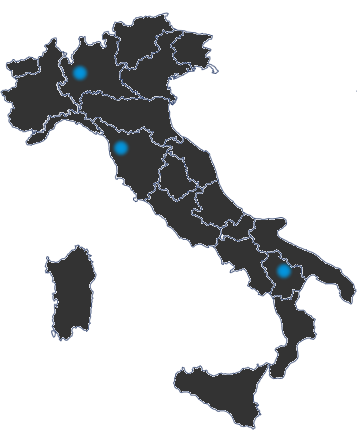
\includegraphics[scale=0.25]{img/italia.png}
%    ~
  \section{Personality}
  	{ISTJ}
    \textbf{Introverted  }
\includegraphics[scale=0.07]{img/3heart.png}
    \textbf{Observant  }
\includegraphics[scale=0.07]{img/1heart.png}
    \textbf{Thinking  }
\includegraphics[scale=0.07]{img/2heart.png}
    \textbf{Judging  }
\includegraphics[scale=0.07]{img/3heart.png}
    \textbf{Assertive  }
\includegraphics[scale=0.07]{img/3heart.png}    
    ~
  \section{Languages}
    \textbf{Chinese  }
\includegraphics[scale=0.07]{img/3heart.png}
    \textbf{English  }
\includegraphics[scale=0.07]{img/2heart.png}
\end{aside}

\section{Projects Details }
\textbf{Blackboard\\}
foo\\
~
\textbf{Sunshine\\}
bar\\
~
\textbf{House Keeper\\}
boo\\
~
\textbf{Lisp Compiler\\}
mii\\
~
\section{Other Info}
For the Italian job market:\\
\emph{Si autorizza il trattamento delle informazioni contenute nel curriculum in conformità alle disposizioni previste dal d.lgs. 196/2003. Si dichiara altresì di essere consapevole che, in caso di dichiarazioni non veritiere, si è passibili di sanzioni penali ai sensi del DPR 445/00 oltre alla revoca dei benefici eventualmente percepiti.}
\\
\begin{flushleft}
\emph{January 14th, 2014}
\end{flushleft}
\begin{flushright}
\emph{Carmine Benedetto}
\end{flushright}

%%% This piece of code has been commented by Karol Kozioł due to biblatex errors. 
% 
%\printbibsection{article}{article in peer-reviewed journal}
%\begin{refsection}
%  \nocite{*}
%  \printbibliography[sorting=chronological, type=inproceedings, title={international peer-reviewed conferences/proceedings}, notkeyword={france}, heading=subbibliography]
%\end{refsection}
%\begin{refsection}
%  \nocite{*}
%  \printbibliography[sorting=chronological, type=inproceedings, title={local peer-reviewed conferences/proceedings}, keyword={france}, heading=subbibliography]
%\end{refsection}
%\printbibsection{misc}{other publications}
%\printbibsection{report}{research reports}

\end{document}
